\usetikzlibrary{arrows.meta,calc,matrix,patterns,shapes}
\providecommand{\computer}{%
    
\includegraphics[width=1cm]{../common/Noun_project_216.pdf}
}
\providecommand{\switch}{%
    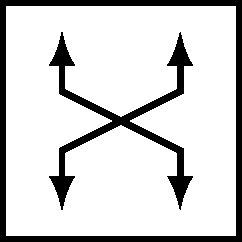
\includegraphics[width=0.9cm]{../common/fig-switch.pdf}
}
\providecommand{\bigswitch}{%
    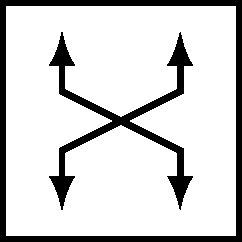
\includegraphics[width=1.4cm]{../common/fig-switch.pdf}
}
\providecommand{\router}{%
    
\includegraphics[width=0.9cm]{../common/fig-router.pdf}
}



\begin{frame}[fragile]{multiprotocol label switching (MPLS)}
    \begin{itemize}
    \item MPLS: combines encapsulation and routing tables
    \end{itemize}
\begin{tikzpicture}
\tikzset{
    box/.style={draw,thick},
    box unused/.style={draw,thick,pattern=north west lines},
    box label/.style={midway,font=\small,align=center},
    computer/.style={inner sep=0mm,outer sep=0mm,execute at begin node={\computer}},
    switch/.style={inner sep=0mm,outer sep=0mm,execute at begin node={\switch}},
    router/.style={inner sep=-.5mm,outer sep=0mm,execute at begin node={\router}},
    port/.style={pos=0.95,fill=white,circle,draw,inner sep=0mm},
    port beginning/.style={pos=0.05,fill=white,circle,draw,inner sep=0mm},
    box label flags/.style={midway,font=\fontsize{8}{9}\selectfont,align=center},
    hi on/.style={alt=<#1>{ultra thick,fill=red!10}},
    explain box 1/.style={draw=red,line width=0.8mm,fill=white,anchor=center,at={(explain box loc 1)},align=center},
    explain box 2/.style={draw=red,line width=0.8mm,fill=white,anchor=center,at={(explain box loc 2)},align=center},
    explain box 3/.style={draw=red,line width=0.8mm,fill=white,anchor=center,at={(explain box loc 3)},align=center},
    route table/.style={
        matrix of nodes,ampersand replacement=\&,
        column sep=-.3mm, row sep=-.3mm,
        nodes={align=center,font=\fontsize{9}{10}\selectfont\tt,text depth=1mm,text height=3mm,minimum height=0.4cm,inner sep=0mm,draw,line width=.3mm},
        column 1/.style={nodes={text width=.7cm}},
        column 2/.style={nodes={text width=0.7cm}},
        column 3/.style={nodes={text width=1.7cm,font=\fontsize{7}{8}\selectfont\tt}},
        column 4/.style={nodes={text width=1.5cm}},
        column 5/.style={nodes={text width=.5cm}},
        row 1/.style={nodes={draw=none,font=\fontsize{9}{10}\selectfont}},
    },
    route table no in no dest/.style={
        matrix of nodes,ampersand replacement=\&,
        column sep=-.3mm, row sep=-.3mm,
        nodes={align=center,font=\fontsize{9}{10}\selectfont\tt,text depth=1mm,text height=3mm,minimum height=0.4cm,inner sep=0mm,draw,line width=.3mm},
        column 1/.style={nodes={text width=0.7cm}},
        column 2/.style={nodes={text width=1.5cm}},
        column 3/.style={nodes={text width=.5cm}},
        row 1/.style={nodes={draw=none,font=\fontsize{9}{10}\selectfont}},
    },
    route table no dest no in/.style={route table no in no dest},
    connect/.style={draw,very thick},
    msg/.style={
        matrix of nodes,nodes={draw,violet,line width=.3mm,font=\fontsize{8}{9}\selectfont\tt,
            inner sep=0mm,inner xsep=.5mm,text height=3mm,text depth=.5mm},
        fill=white,
        column sep=-.3mm,inner sep=0mm
    },
    >=Latex,
    hi row/.style 2 args={
        alt=<#1>{
            row #2/.style={nodes={fill=red!15}}
        }
    },
}
\node[router] (in0) at (0, 6) {};
\draw[connect,->] (-1, 7) -- (in0.north west) node[port]{0};
%\draw[connect,->] (-1, 6) -- (in0.west) node[port]{1};
\matrix[route table,anchor=north,hi row={2}{2}] at (0, 5.5) {
in \& label \& dest \& op \& out \\
0\& --- \& 3fff:1::/32 \& push 4 \& 2 \\
0 \& --- \& 3fff:2::/32 \& push 7 \& 2 \\
2 \& 9 \& --- \& pop \& 0\\
\ldots \& \ldots \& \ldots \& \ldots \& \ldots \\
};
\node[router] (out0) at (10, 8) {};
\draw[connect,->] (out0.east) -- ++(.5, 0) node[right,font=\tiny\tt] {3fff:1::/32}
    node[port beginning] {1};
\draw[connect,->] (out0.north east) -- ++(.5, .5)
    node[port beginning] {2};
\node[router] (out1) at (5, 4) {};
\draw[connect,->] (out1.south) -- ++(0, -.5) node[right,font=\tiny\tt] {3fff:2::/32}
    node[port beginning] {1};
\node[router,alt=<5>{fill=red!10}] (mid1) at (5, 6) {};
\matrix[alt=<5>{draw=red,very thick},route table no in no dest,anchor=south,hi row={2-4}{2}] (mid1 table) at ([xshift=-1.5cm]mid1.north) {
label \& op \& out \\
24 \& swap 1 \& 21 \\
25 \& swap 2 \& 21 \\
27 \& swap 1 \& 22 \\
28 \& swap 9 \& 0 \\
\ldots \& \ldots \& \ldots \\
};
\matrix[route table,anchor=north,hi row={2}{4}] at ([yshift=-.3cm]out0.south) {
in \& label \& dest \& op \& out \\
1 \& --- \& 3fff:2::/32\& push 27 \& 0\\
1 \& --- \& default \& push 28 \& 0\\
0 \& 21 \& --- \& pop \& 21 \\
0 \& 22 \& --- \& pop \& 22 \\
\ldots \& \ldots \& \ldots \& \ldots \& \ldots \\
};
\foreach \x/\y/\xp/\yp in {in0/mid1/2/0,mid1/out0/1/0,mid1/out1/2/0} {
    \draw[connect,<->] (\x) -- (\y) node[port beginning] {\xp} node[port] {\yp};
}
\begin{visibleenv}<2-4>
    \matrix[msg,anchor=south] at ([yshift=.5cm]in0.north west) {
        dest=3fff:1::aa \& \ldots \\
    };
    \matrix[msg,anchor=west] at ([xshift=.5cm]in0.east) {
        |[alt={<3>{fill=red!15}}]| 24 \& dest=3fff:1::aa \& \ldots \\
    };
    \matrix[msg,anchor=west] at ([xshift=.5cm,yshift=1cm]mid1.east) {
        |[alt={<3>{fill=red!15}}]| 21 \& dest=3fff:1::aa \& \ldots \\
    };
\end{visibleenv}
\begin{visibleenv}<3>
\node[align=left,draw=red,very thick,fill=white,anchor=west] at (mid1 table.east) {
    `swap' operation to translate \\
    between different label meanings \\
    ~ \\
    allows piecemail configuration
};
\end{visibleenv}
\begin{visibleenv}<5>
\node[align=left,draw=red,very thick,fill=white,anchor=west] at (mid1 table.east) {
    routers in `middle' of network \\
    have \textit{very simple} routing decisions \\
    no prefix matching
};
\end{visibleenv}
\end{tikzpicture}
\end{frame}

\begin{frame}{Label Distribution Protocol}
    \begin{itemize}
    \item share with neighbors list of:
        \begin{itemize}
        \item (ultimate destination, desired label)
        \end{itemize}
    \item use entries to
        \begin{itemize}
        \item allocate new local labels
        \item setup appropriate \texttt{swap} entries
        \item send other neighbors update about new labels
        \end{itemize}
    \vspace{.5cm}
    \item if using normal routing protocol to decide which neighbors routes to accept,
    just a funny way to implement routing tables
    \end{itemize}
\end{frame}

\begin{frame}[fragile]{MPLS tunnel}
\begin{tikzpicture}
\tikzset{
    box/.style={draw,thick},
    box unused/.style={draw,thick,pattern=north west lines},
    box label/.style={midway,font=\small,align=center},
    computer/.style={inner sep=0mm,outer sep=0mm,execute at begin node={\computer}},
    switch/.style={inner sep=0mm,outer sep=0mm,execute at begin node={\switch}},
    router/.style={inner sep=-.5mm,outer sep=0mm,execute at begin node={\router}},
    port/.style={pos=0.95,fill=white,circle,draw,inner sep=0mm},
    port beginning/.style={pos=0.05,fill=white,circle,draw,inner sep=0mm},
    box label flags/.style={midway,font=\fontsize{8}{9}\selectfont,align=center},
    hi on/.style={alt=<#1>{ultra thick,fill=red!10}},
    explain box 1/.style={draw=red,line width=0.8mm,fill=white,anchor=center,at={(explain box loc 1)},align=center},
    explain box 2/.style={draw=red,line width=0.8mm,fill=white,anchor=center,at={(explain box loc 2)},align=center},
    explain box 3/.style={draw=red,line width=0.8mm,fill=white,anchor=center,at={(explain box loc 3)},align=center},
    route table/.style={
        matrix of nodes,ampersand replacement=\&,
        column sep=-.3mm, row sep=-.3mm,
        nodes={align=center,font=\fontsize{9}{10}\selectfont\tt,text depth=1mm,text height=3mm,minimum height=0.4cm,inner sep=0mm,draw,line width=.3mm},
        column 1/.style={nodes={text width=.7cm}},
        column 2/.style={nodes={text width=0.7cm}},
        column 3/.style={nodes={text width=1.7cm,font=\fontsize{7}{8}\selectfont\tt}},
        column 4/.style={nodes={text width=1.5cm}},
        column 5/.style={nodes={text width=.5cm}},
        row 1/.style={nodes={draw=none,font=\fontsize{9}{10}\selectfont}},
    },
    route table no in no dest/.style={
        matrix of nodes,ampersand replacement=\&,
        column sep=-.3mm, row sep=-.3mm,
        nodes={align=center,font=\fontsize{9}{10}\selectfont\tt,text depth=1mm,text height=3mm,minimum height=0.4cm,inner sep=0mm,draw,line width=.3mm},
        column 1/.style={nodes={text width=0.7cm}},
        column 2/.style={nodes={text width=1.5cm}},
        column 3/.style={nodes={text width=.5cm}},
        row 1/.style={nodes={draw=none,font=\fontsize{9}{10}\selectfont}},
    },
    route table no dest/.style={
        matrix of nodes,ampersand replacement=\&,
        column sep=-.3mm, row sep=-.3mm,
        nodes={align=center,font=\fontsize{9}{10}\selectfont\tt,text depth=1mm,text height=3mm,minimum height=0.4cm,inner sep=0mm,draw,line width=.3mm},
        column 1/.style={nodes={text width=0.7cm}},
        column 2/.style={nodes={text width=0.7cm}},
        column 3/.style={nodes={text width=1.5cm}},
        column 4/.style={nodes={text width=.5cm}},
        row 1/.style={nodes={draw=none,font=\fontsize{9}{10}\selectfont}},
    },
    route table no dest no in/.style={route table no in no dest},
    connect/.style={draw,very thick},
    msg/.style={
        matrix of nodes,nodes={draw,violet,line width=.3mm,font=\fontsize{8}{9}\selectfont\tt,
            inner sep=0mm,inner xsep=.5mm,text height=3mm,text depth=.5mm},
        fill=white,
        column sep=-.3mm,inner sep=0mm},
    >=Latex,
    hi row/.style 2 args={
        alt=<#1>{
            row #2/.style={nodes={fill=red!15}}
        }
    },
}

\node at (6, 9) {logical view --- `virtual wire'};
\node (log A) at (-2, 8.5) {A};
\node (log B) at (13, 8.5) {B};
\draw[connect,<->] (log A) -- (log B);

\draw[overlay, ultra thick] (-3.5, 7.8) -- (14, 7.8);

\node[anchor=north] at (6, 7.8) {actual network};

\node[router] (in0) at (0, 6) {};
\draw[connect,<->] (-1.5, 6) -- (in0.west) node[port]{0}
    node[pos=0,left] {A};
\matrix[route table no dest,anchor=north] at (0, 5.5) {
in \& label  \& op \& out \\
0 \& ---  \& push 32 \& 1 \\
--- \& 1 \& pop \& 0 \\
\ldots \& \ldots \& \ldots \& \ldots \\
};
\node[router] (mid1) at (4, 6) {};
\matrix[route table no dest no in,anchor=north] at (4, 4) {
label  \& op \& out \\
32 \& swap 37 \& 4 \\
26 \& swap 21 \& 0 \\
\ldots \& \ldots \& \ldots \\
};
\node[router] (mid2) at (8, 6) {};
\matrix[route table no dest no in,anchor=north] at (8, 5.5) {
label  \& op \& out \\
37 \& swap 20 \& 6 \\
39 \& swap 32 \& 3 \\
\ldots \& \ldots \& \ldots \\
};
\node[router] (out0) at (11, 6) {};
\matrix[route table no dest,anchor=north] at (11, 4) {
in \& label  \& op \& out \\
0 \& --- \& push 37 \& 1 \\
--- \& 0 \& swap 29 \& 6 \\
\ldots \& \ldots \& \ldots \& \ldots \\
};
\draw[connect,->](out0.east) -- ++(1, 0) node[port beginning]{0}
    node[pos=1,right] {B};

\foreach \x/\y in {mid1/30,mid1/60,mid1/270,mid2/45,mid2/90,mid2/210,mid2/290,
                   in0/90,in0/270,out0/60,out0/280} {
    \draw[connect,<-] (\x.\y) -- ++(\y:.5cm);
};
\foreach \x/\y/\xp/\yp in {in0/mid1/1/0,mid1/mid2/4/3,mid2/out0/6/1} {
    \draw[connect,<->] (\x) -- (\y) node[port beginning] {\xp} node[port] {\yp};
}
\end{tikzpicture}
\end{frame}

\begin{frame}{MPLS tunnels for traffic engineering}
    \begin{itemize}
    \item if multiple paths from A to B often want to:
        \begin{itemize}
        \item balance between them to use available bandwidth
        \item prioritize important traffic on `better' path
        \item \ldots
        \end{itemize}
    \item plain OSPF can't really do any of this unless equal cost
    \vspace{.5cm}
    \item MPLS gives mechanism to do this kind of balancing:
        \begin{itemize}
        \item setup labels along desired paths
        \item choosing new path (or failover) = changing `swap X' to `swap Y'
        \item can configure backup paths in advance and turn them on later
        \end{itemize}
    \end{itemize}
\end{frame}

\begin{frame}[fragile]{rapid failover}
\begin{tikzpicture}
\tikzset{
    box/.style={draw,thick},
    box unused/.style={draw,thick,pattern=north west lines},
    box label/.style={midway,font=\small,align=center},
    computer/.style={inner sep=0mm,outer sep=0mm,execute at begin node={\computer}},
    switch/.style={inner sep=0mm,outer sep=0mm,execute at begin node={\switch}},
    router/.style={inner sep=-.5mm,outer sep=0mm,execute at begin node={\router}},
    port/.style={pos=0.95,fill=white,circle,draw,inner sep=0mm},
    port beginning/.style={pos=0.05,fill=white,circle,draw,inner sep=0mm},
    box label flags/.style={midway,font=\fontsize{8}{9}\selectfont,align=center},
    hi on/.style={alt=<#1>{ultra thick,fill=red!10}},
    explain box 1/.style={draw=red,line width=0.8mm,fill=white,anchor=center,at={(explain box loc 1)},align=center},
    explain box 2/.style={draw=red,line width=0.8mm,fill=white,anchor=center,at={(explain box loc 2)},align=center},
    explain box 3/.style={draw=red,line width=0.8mm,fill=white,anchor=center,at={(explain box loc 3)},align=center},
    route table/.style={
        matrix of nodes,ampersand replacement=\&,
        column sep=-.3mm, row sep=-.3mm,
        nodes={align=center,font=\fontsize{9}{10}\selectfont\tt,text depth=1mm,text height=3mm,minimum height=0.4cm,inner sep=0mm,draw,line width=.3mm},
        column 1/.style={nodes={text width=.7cm}},
        column 2/.style={nodes={text width=0.7cm}},
        column 3/.style={nodes={text width=1.7cm,font=\fontsize{7}{8}\selectfont\tt}},
        column 4/.style={nodes={text width=1.5cm}},
        column 5/.style={nodes={text width=.5cm}},
        row 1/.style={nodes={draw=none,font=\fontsize{9}{10}\selectfont}},
    },
    route table no in no dest/.style={
        matrix of nodes,ampersand replacement=\&,
        column sep=-.3mm, row sep=-.3mm,
        nodes={align=center,font=\fontsize{9}{10}\selectfont\tt,text depth=1mm,text height=3mm,minimum height=0.4cm,inner sep=0mm,draw,line width=.3mm},
        column 1/.style={nodes={text width=0.7cm}},
        column 2/.style={nodes={text width=1.5cm}},
        column 3/.style={nodes={text width=.5cm}},
        row 1/.style={nodes={draw=none,font=\fontsize{9}{10}\selectfont}},
    },
    route table no dest/.style={
        matrix of nodes,ampersand replacement=\&,
        column sep=-.3mm, row sep=-.3mm,
        nodes={align=center,font=\fontsize{9}{10}\selectfont\tt,text depth=1mm,text height=3mm,minimum height=0.4cm,inner sep=0mm,draw,line width=.3mm},
        column 1/.style={nodes={text width=0.7cm}},
        column 2/.style={nodes={text width=0.7cm}},
        column 3/.style={nodes={text width=1.5cm}},
        column 4/.style={nodes={text width=.5cm}},
        row 1/.style={nodes={draw=none,font=\fontsize{9}{10}\selectfont}},
    },
    route table no dest no in/.style={route table no in no dest},
    connect/.style={draw,very thick},
    msg/.style={
        matrix of nodes,nodes={draw,violet,line width=.3mm,font=\fontsize{8}{9}\selectfont\tt,
            inner sep=0mm,inner xsep=.5mm,text height=3mm,text depth=.5mm},
        fill=white,
        column sep=-.3mm,inner sep=0mm},
    >=Latex,
    hi row/.style 2 args={
        alt=<#1>{
            row #2/.style={nodes={fill=red!15}}
        }
    },
}

\draw[connect,<->] (-1.5, 6) -- (in0.west) node[port]{0}
\node[router] (in0) at (0, 6) {};
\matrix[route table no dest no  in,anchor=north] at (0, 5.5) {
label  \& op \& out \\
21 \& swap 25 \& 1 \\
(backup) 21 \& swap 27 \& 2 \\
27 \& swap 30 \& 0 \\
 \ldots \& \ldots \& \ldots \\
};
\node[router] (mid1) at (12, 6) {};
\matrix[route table no dest no in,anchor=north] at (12, 5.5) {
label  \& op \& out \\
25 \& swap 27 \& 3 \\ 
 \ldots \& \ldots \& \ldots \\
};
\node[router] (out0) at (6, 4) {};
\matrix[route table no dest no in,anchor=north] at (6, 3.5) {
label  \& op \& out \\
27 \& swap 24 \& 3 \\
28 \& swap 25 \& 1 \\
\ldots \& \ldots \& \ldots \\
};
\draw[connect,<->] (-13.5, 6) -- (out0.east) node[port]{1}
\foreach \x/\y/\xp/\yp in {in0/out0/1/1,in0/mid1/2/1,mid1/out0/3/2} {
    \draw[connect,<->] (\x) -- (\y) node[port beginning] {\xp} node[port] {\yp};
}
\end{tikzpicture}
\end{frame}

\begin{frame}{RSVP-TE}
    \begin{itemize}
    \item RSVP-TE (RFC 3209): protocol for setting up MPLS tunnels
    \item idea: routers figure out labels, etc.
    \item end-user can (optionally) specify\ldots
    \vspace{.5cm}
    \item that tunnel go through specific routers
    \item also setting up `fast reroute' backup paths
    \item bandwidth reservation 
        \begin{itemize}
        \item routers give you error if bandwidth not gaurenteed
        \end{itemize}
    \end{itemize}
\end{frame}

\begin{frame}{nested labels}
    \begin{itemize}
    \item label \textit{stack} allows \ldots
    \item nested tunnels
    \item marking different types of packet
    \item \ldots
    \end{itemize}
\end{frame}

\begin{frame}{protocol-independence}
    \begin{itemize}
    \item only first/last routers care about actual protocol
    \item easily allows for\ldots
    \vspace{.5cm}
    \item mix of Ethernet and IP tunnels
    \item using routers that don't support IP (e.g. ATM)
    \item \ldots
    \end{itemize}
\end{frame}

\begin{frame}[fragile]{actual label format}
\begin{Verbatim}[fontsize=\small]
 0                   1                   2                   3
 0 1 2 3 4 5 6 7 8 9 0 1 2 3 4 5 6 7 8 9 0 1 2 3 4 5 6 7 8 9 0 1
+-+-+-+-+-+-+-+-+-+-+-+-+-+-+-+-+-+-+-+-+-+-+-+-+-+-+-+-+-+-+-+-+ Label
|                Label                  | Exp |S|       TTL     | Stack
+-+-+-+-+-+-+-+-+-+-+-+-+-+-+-+-+-+-+-+-+-+-+-+-+-+-+-+-+-+-+-+-+ Entry

                    Label:  Label Value, 20 bits
                    Exp:    Experimental Use, 3 bits
                    S:      Bottom of Stack, 1 bit
                    TTL:    Time to Live, 8 bits
\end{Verbatim}
\begin{itemize}
\item TTL here is different than we've seen:
\item only processed when label popped
\item typically (re)set to mirror IP TTL if MPLS run over IP
\end{itemize}
\end{frame}


